\chapter{Identical Particles}

Due to Heisenberg uncertainty principle, it is impossible to keep track of individual particles. Due to uncertainty principle, $\Delta x \Delta p \geq \frac{\hbar}{2}$, if we try to localize two particles within a region $\Delta x$ small enough then it is impossible to distinguish their momenta, i.e. the direction and magnitude of their velocities as shown in . Thus, even if we label two particles as 1 and 2 at time $t=0$, after some time we cannot say which particle is which.
\begin{figure}[h!]
    \centering
    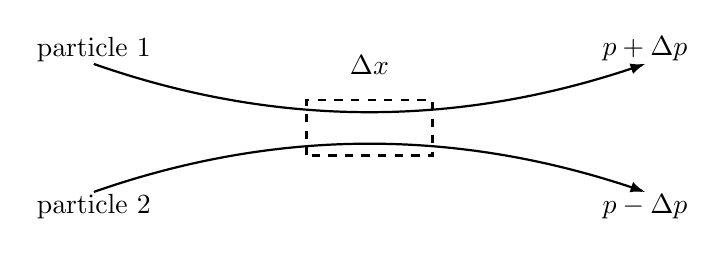
\begin{tikzpicture}[x=1cm,y=1cm,>=latex]


  % Two "wide" parabolas: one opening up, one opening down
  % Tune coefficients to make them "less curved" (small curvature).
  \draw[thick,->]
    plot[domain=0:7,samples=200]
    (\x,{0.05*(\x-3.5)^2 + 0.2});

  \draw[thick,->]
    plot[domain=0:7,samples=200]
    (\x,{-0.05*(\x-3.5)^2 - 0.2});

  % Region where they get close: dashed rectangle
  % Adjust these numbers to cover the "closest" part you want.
  \draw[dashed, thick] (2.7,-0.35) rectangle (4.3,0.35);
    \node at (0,1) {particle 1};
    \node at (0,-1) {particle 2};
    \node at (3.5,0.8) {$\Delta x$};
    \node at (7,1) {$p + \Delta p$};
    \node at (7,-1) {$p - \Delta p$};
\end{tikzpicture}
\caption{If spatial resolution is good enough to distinguish the two particles well enough, then we can not say which one goes up and down after the scattering. Also, if the momentum resolution is good enough}
\end{figure}
\section{Bosons and Fermions}

Consider $N$ identical particles (e.g., electrons, $\pi$ mesons). The Hamiltonian 
\begin{align}
    \oH = \oH(\xi_1,\xi_2,\dots,\xi_N)
\end{align}
is symmetric in the variables $\xi_1,\xi_2,\dots$. Here these variables includes position and spin degrees of freedom ($\bfvec{x}_i,\chi_{i}$ for $i=1,2,\dots,N$)\footnote{Even some other internal degrees of freedom such as isospin, color, flavor}. Likewise, we write a wave function in the form 
\begin{align}
    \psi = \psi(\xi_1,\xi_2,\dots,\xi_N)
\end{align}

Define a permutation operator (also called exchange operator) $\oP_{ij}$ as an operator that, when acting on an arbitrary $N-$particle wave function is 
\begin{align}
    \oP_{ij} \psi(\xi_1,\dots,\xi_i,\dots,\xi_j,\dots,\xi_N) = \psi(\xi_1,\dots,\xi_j,\dots,\xi_i,\dots,\xi_N)
\end{align}
By this we can see
\begin{align}
    \oP_{ij}^2 \psi(\dots) = \oP_{ij} \psi(\dots, i \leftrightarrow j) = \psi(\dots)
\end{align}
which means that\footnote{But we must be careful, the operator act the whole Hilbet space, such that this result is always true }
\begin{align}
    \oP^2_{ij} = \oI 
\end{align}
The eigenvalue of the permutation operator is $\pm 1$, which is obtained from following:
\begin{align*}
    &\oP_{ij} \phi = \lambda \phi \quad \forall \phi \neq 0 \\
   \implies& \oP^2{ij} \phi = \phi = \lambda^2 \phi  \\
    \implies & \lambda^2 = 1 , \quad \lambda = \pm1 \\
    \implies &\oP_{ij} \psi(\xi_1,\dots,\xi_i,\dots,\xi_j,\dots \xi_N) = \pm \psi(\xi_1,\dots,\xi_i,\dots,\xi_j,\dots \xi_N)
\end{align*}
Such that we can find that the eigenfunctions corresponding to the eigenvalue of $+1$ are symmetric and those corresponding to $-1$ corresponding to $-1$ are antisymmetric with respect to interchange of the pair $(i,j)$. Denoting by $\psi_{s} $ and $\psi_a$
\begin{align}
    \psi_s (\xi_1,\dots,\xi_i,\dots,\xi_j,\dots,\xi_N) &= + \psi_s (\xi_1,\dots,\xi_j,\dots,\xi_i,\dots,\xi_N) \\
    \psi_a (\xi_1,\dots,\xi_i,\dots,\xi_j,\dots,\xi_N) &= - \psi_a (\xi_1,\dots,\xi_j,\dots,\xi_i,\dots,\xi_N)
\end{align}

As we have discussed before,  identical particles are indistinguishable. Such that if the permutation of two particles does not change the physical observables, this implies that the Hamiltonian is symmetric with respect to the interchange of any pair of particles, i.e., $\comm{\oH}{\oP_{ij}} = 0$.
\paragraph{Properties of the permutation operator}
\begin{enumerate}
    \item If $\psi(\xi_1,\dots , \xi_N)$ is an eigenfunction of $\oH$ with eigenvalue $\oH$ with eigenvalue $E$, then the same also holds for $\oP_{ij} \psi(\xi_1,\dots,\xi_N)$.
    \begin{proof}
        \begin{align*}
            \oH \oP_{ij} \psi &= \oP_{ij} \oH \psi \\
            &= E \oP_{ij} \psi
        \end{align*}
    \end{proof}
    \item For every permutation one has 
    \begin{align}
        \braket{\Phi|\Psi} = \bra{\Phi} \oP_{ij}^\dagger \oP_{ij} \ket{\Psi} = \braket{\oP_{ij} \Phi | \oP_{ij} \Psi}
    \end{align}
    This comes from the fact that the permutation operator just changes the labels of the integration variables in the inner product integral. This also indicates that the permutation operator is unitary, i.e.,
    \begin{align}
        \oP_{ij}^\dagger \oP_{ij} = \oI
    \end{align}
    \item For every symmetric operator $\oS(\xi_1,\dots,\xi_N)$ we have 
    \begin{align}
        \comm{\oS}{\oP_{ij}} = 0
    \end{align}
    and 
    \begin{align}
        \bra{\psi_i} \oS \ket{\psi_j} = \bra{\oP_{ij} \psi_i} \oS \ket{\oP_{ij} \psi_j}
    \end{align}
\end{enumerate}

If we say that the particles are indistinguishable, then the physical observables should not change under the action of the permutation operator, consider two particles, with two observables $\oA_1$ and $\oA_2$, 

\begin{align}
    \oP_{ij} \oA \oP_{ij} = \oA
\end{align}
This implies that the Hamiltonian commutes with the permutation operator,
\begin{align}
    [\oH, \oP_{ij}] = 0
\end{align}

Particles described by symmetric wave functions are called bosons, while those described by antisymmetric wave functions are called fermions. Examples of bosons include photons, W and Z bosons, gluons, and the Higgs boson. Examples of fermions include electrons, protons, neutrons, and quarks.















